% !TEX program = pdflatex
% compilar con pdflatex (2 pasadas) desde esta carpeta (informe/)
\documentclass[11pt,a4paper]{article}

\usepackage[utf8]{inputenc}
\usepackage[T1]{fontenc}
\usepackage[spanish,es-tabla]{babel}
\usepackage[margin=2.4cm]{geometry}
\usepackage{amsmath,amssymb}
\usepackage{booktabs}
\usepackage{graphicx}
\usepackage{xcolor}
\usepackage{float}
\usepackage{enumitem}
\usepackage[colorlinks=true,linkcolor=blue!60!black,citecolor=blue!60!black,urlcolor=blue!60!black]{hyperref}

\graphicspath{{../analisis/figs/}}

% numeros medidos en el notebook (los actualizo a mano cuando lo vuelvo a correr)
\newcommand{\SIGeff}{0.229}
\newcommand{\DIVBfin}{2.3\times10^{-1}}
\newcommand{\EDRIFT}{7\times10^{-11}}

\title{\textbf{Proyecto 2 — extensión 3D: inestabilidad Rayleigh--Taylor magnetizada
como modelo local de la interfaz de un remanente de supernova}\\[4pt]
\large corrida PLUTO del setup \texttt{Rayleigh\_Taylor} (config \#09) + análisis}
\author{Zeuz Espinosa\\ Astrof\'isica Computacional 2026-II}
\date{Noviembre de 2026}

\begin{document}
\maketitle

\section{De qué se trata esto y qué quería entender}

La parte principal del proyecto es la RT magnetizada 2D (config \#07 de
\texttt{Rayleigh\_Taylor}, ver la guía en \texttt{Rayleigh\_Taylor\_MHD/}). Esta carpeta es
la extensión que quise hacer por el lado astrofísico: el mismo setup pero en
\textbf{3D} y con perturbación aleatoria. La pregunta que me guía es la de las fotos de
Tycho y Cas~A: se ven ``dedos'' de eyecta penetrando el medio circundante, y la literatura
dice que el campo magnético ambiental los frena y los alarga \cite{orlando2012,
fraschetti2010}. Quería ver si con mi computador puedo \emph{reproducir esa física}:
hacer que aparezcan dedos, medir qué tan rápido crecen, y comprobar que el campo los deja
anisótropos (alargados a lo largo de las líneas).

Escribir esto me sirvió para entender varias cosas que en el notebook quedan implícitas,
así que el informe sigue más o menos el orden en que yo fui entendiendo el problema:
primero por qué una interfaz acelerada ``es'' una RT (\S2), después qué decidí correr y
por qué (\S3), qué dice la teoría que debería salir (\S4), qué salió (\S5) y qué no
alcanzó (\S6). Todo el material (corrida, notebook, datos) está en \texttt{SNR\_3D/};
el notebook ejecutado es \texttt{analisis/SNR\_3D\_analisis.ipynb}.

\section{Por qué una RT plana ``es'' un pedazo de SNR}

\subsection{La física: el contacto desacelera}

En la fase de eyecta dominada, el remanente crece como $R(t)=C\,t^\eta$ con $\eta<1$
(Sedov: $\eta=2/5$; Chevalier 1982 para la eyecta con perfil en ley de potencias
\cite{warren2013}). Si derivo dos veces,
\begin{equation}
a=\ddot{R}=\eta(\eta-1)\,\frac{R}{t^2}
\;\;\Longrightarrow\;\;
|a|=\eta(1-\eta)\,\frac{R}{t^2}\,,
\label{eq:geff}
\end{equation}
o sea que la superficie \emph{desacelera}. Eso fue lo que más me costó ver al principio:
la intuición dice ``una explosión se expande cada vez más rápido'', pero en realidad el
SNR barre masa y se frena. Orden de magnitud para Tycho ($R\sim5$ pc, $t\sim430$ yr):
$|a|\sim2\times10^{-4}\ \mathrm{m/s^2}$ --- pequeñísima como aceleración, pero lo
importante no es su tamaño absoluto sino su \emph{dirección} relativa a la estratificación.

Dentro del choque delantero hay dos superficies distintas, y distinguirlas fue clave:
\begin{itemize}[nosep]
  \item el \textbf{choque} mismo: salta la presión, comprime y calienta el medio;
  \item la \textbf{discontinuidad de contacto} entre eyecta chocada y medio chocado:
  misma presión a ambos lados, densidades distintas.
\end{itemize}
En el marco que desacelera junto con el contacto, la ecuación~\eqref{eq:geff} actúa como
una ``gravedad efectiva'' que apunta \emph{del fluido ligero al pesado} (del medio chocado
a la eyecta chocada). Esa es exactamente la condición de Rayleigh--Taylor: fluido pesado
(eyecta, $\rho_2$) ``apoyado'' sobre ligero (medio, $\rho_1$) contra una aceleración. El
contacto ---no el choque--- es lo que se rompe en dedos.

\subsection{El mapa a la simulación}

Con eso, la corrida es un \emph{parche local} del contacto, y cada pieza del setup
corresponde a algo físico:

\begin{table}[H]
\centering\small
\caption{El diccionario SNR $\leftrightarrow$ simulación. Es la tabla que yo hubiera
querido tener al empezar.}
\begin{tabular}{@{}p{5.4cm}p{9.9cm}@{}}
\toprule
En la simulación & En el remanente \\
\midrule
fluido pesado arriba ($\rho_2=\eta=4$) & eyecta chocada (densa) \\
fluido ligero abajo ($\rho_1=1$) & medio circundante chocado \\
$g=-0.01$ constante & desaceleración del contacto (\ref{eq:geff}); en el SNR real decae
con el tiempo, aquí la tomo constante \\
picos que \emph{caen} & dedos de eyecta que penetran hacia afuera \\
burbujas que \emph{suben} & medio chocado que se cuela entre los dedos \\
$\mathbf{B}=B_x\,\hat{\mathbf{x}}$ uniforme & campo ambiental ``drapado'' en el choque
delantero: tangente a la superficie del contacto \\
perturbación aleatoria & el ruido multimodo real de la interfaz (frente corrugado del
choque, clumpiness de la eyecta) \\
\bottomrule
\end{tabular}
\end{table}

Las cantidades NO están en unidades de un SNR real sino en unidades de código del test
problem ($L_x=1$, $\rho_1=1$, $c_{s,1}=1$): lo que busco es la física \emph{cualitativa}
del crecimiento y la anisotropía. El contraste eyecta/ambiente real es mucho mayor que
$\eta=4$ (de decenas a miles); con mayor $A$ los picos caen más cerca de caída libre y
las tasas suben como $\sqrt{A}$, pero el mecanismo es el mismo.

\section{Qué corrí exactamente, y por qué cada cosa}

Configuración \#09 del setup (MHD 3D, RK2, reconstrucción LINEAR con limitador MC,
limpieza de divergencia GLM, solver Roe). La resumo y después explico las decisiones:

\begin{table}[H]
\centering\small
\caption{La corrida en una tabla.}
\begin{tabular}{@{}p{2.5cm}p{12.9cm}@{}}
\toprule
Malla & $48\times96\times48$; $x,z\in[-0.5,0.5]$, $y\in[-1.5,0.5]$ (interfaz en $y=0$) \\
Fronteras & periódicas en $x,z$; reflectivas en $y$ \\
Parámetros & \texttt{ETA=4.0}, \texttt{GRAV=-0.01}, \texttt{CHI=0.2}; $\gamma=5/3$ \\
Campo & $B_x=\chi\sqrt{(\eta-1)|g|}/\sqrt{4\pi}\simeq 9.8\times10^{-3}$ ($\beta\approx1.3\times10^4$) \\
CFL & 0.25; $t_\mathrm{stop}=30$, salidas dbl cada 2.0 (16 archivos) \\
Costo & $\sim$0.22 s/paso serial, $\sim$5800 pasos $\approx$ 22 min \\
\bottomrule
\end{tabular}
\end{table}

\begin{itemize}
  \item \textbf{Perturbación aleatoria} (\texttt{USE\_RANDOM\_PERTURBATION YES}): con la
  semilla gaussiana 3D del setup sale una sola burbuja bonita; con ruido sale una capa de
  mezcla multimodo, que es lo que se ve en las imágenes de Tycho (muchos dedos de muchos
  tamaños compitiendo). Además el ruido siembra \emph{todos} los ángulos de
  $\mathbf{k}$, que es justo lo que necesito para que la anisotropía magnética se pueda
  medir en el espectro (\S5.3).
  \item \textbf{Dominio asimétrico en $y$} ($[-1.5,0.5]$): el autor del test problem le
  da más espacio \emph{abajo}. Los que
  viajan lejos son los \emph{picos} (hacia abajo): son los dedos de eyecta, que es justo
  la parte que quiero que llegue lejos sin chocar con la pared reflectiva.
  \item \textbf{GLM y no CT}: la config \#09 (3D) trae limpieza GLM; la \#07 (2D) trae
  transporte restringido. La diferencia práctica aparece en \S5.4: GLM deja un residuo
  pequeño de $\nabla\cdot\mathbf{B}$ (los errores se propagan y amortiguan, pero no se
  anulan exactamente como en CT). Acepto ese precio porque es la configuración 3D
  probada del setup.
  \item \textbf{CFL 0.25}: más conservador que el 0.8 de la 2D, porque GLM agrega al
  sistema una onda extra (la que barre los errores de divergencia) y el esquema RK2 con
  reconstrucción lineal prefiere margen. Con $\Delta t\approx0.25\,\Delta x/c_f$ y
  $c_f\approx c_s=1$: $\Delta t\approx5\times10^{-3}$.
  \item \textbf{El parche del \texttt{init.c}}: con la perturbación aleatoria activada,
  el \texttt{init.c} original llama \texttt{Random\allowbreak Number()} sin sembrar la secuencia y
  PLUTO aborta con ``\texttt{maximum number of prns exceeded}''. El fix es de 5 líneas:
  un \texttt{static int first\_call} que llama \texttt{Random\allowbreak Seed\allowbreak(26041988,\allowbreak 0)} la primera
  vez. Semilla fija = corrida reproducible (si la cambio, los dedos cambian de lugar pero
  las estadísticas no).
\end{itemize}

\section{Qué dice la teoría que debería salir}

Con el campo en $\hat{x}$, la relación de dispersión de Chandrasekhar
\cite{chandra1961} para una perturbación $\propto e^{i(k_x x+k_z z)+\sigma t}$ (unidades
de PLUTO, sin $4\pi$) es
\begin{equation}
\sigma^2 = \underbrace{A\,g\,k}_{\text{flotabilidad}}
-\underbrace{\frac{2(k_xB)^2}{\rho_1+\rho_2}}_{\text{tensión magnética}},
\qquad k=\sqrt{k_x^2+k_z^2},\quad A=\tfrac{3}{5}.
\label{eq:disp}
\end{equation}
La leí muchas veces hasta separarla en sus dos ideas:
\begin{enumerate}
  \item \textbf{Solo $k_x$ siente el campo}. El término de tensión entra con
  $(\mathbf{k}\cdot\mathbf{B})=k_xB$. Un modo con $\mathbf{k}\perp\mathbf{B}$ (variación
  solo en $z$) no estira las líneas: las desplaza en bloque. Esos ``modos de intercambio'' crecen como en hidrodinámica pura.
  En 2D todo modo era paralelo a $\mathbf{B}$ (máxima supresión); en 3D conviven ambos
  tipos, y de esa convivencia sale la anisotropía que quiero medir.
  \item \textbf{La tensión es como una cuerda}: cada lado de la interfaz aporta su
  tensión; por eso el factor 2. Cuando la tensión le gana a la flotabilidad, el modo
  está estabilizado.
\end{enumerate}

Números del caso (salen de \texttt{teoria\_snr.py}, que además dibuja el mapa completo
$\sigma(k_x,k_z)$):

\begin{table}[H]
\centering\small
\caption{Predicciones lineales para $\eta=4$, $g=0.01$, $\chi=0.2$, $L_x=1$.}
\begin{tabular}{@{}p{6.2cm}p{3.2cm}p{5.8cm}@{}}
\toprule
Cantidad & Valor & Qué me dice \\
\midrule
Atwood $A$ & 0.6 & asimetría fuerte: picos $\gg$ burbujas en velocidad \\
$B_x$; $\beta$ & $9.8\times10^{-3}$; $1.3\times10^4$ & campo débil en presión: no deforma
el equilibrio, actúa por tensión \\
corte paralelo $\lambda_c=\chi^2L_x$ & 0.04 & modos $\parallel$B más cortos que esto no crecen \\
máximo paralelo $\sigma^{\max}_\parallel$ & 0.485 en $\lambda=0.08$ & el modo paralelo
más inestable que existe \\
fundamental diagonal ($k_x=k_z=2\pi$) & 0.228 & el modo más largo que cabe en la caja \\
intercambio puro ($k_x=0$, mismo $k$) & 0.194 & sin freno magnético \\
Nyquist $k_\mathrm{Nyq}=\pi/\Delta x$ & $\approx151$ ($\lambda=0.042$) & lo más fino que
la malla puede representar \\
\bottomrule
\end{tabular}
\end{table}

\begin{figure}[H]
\centering
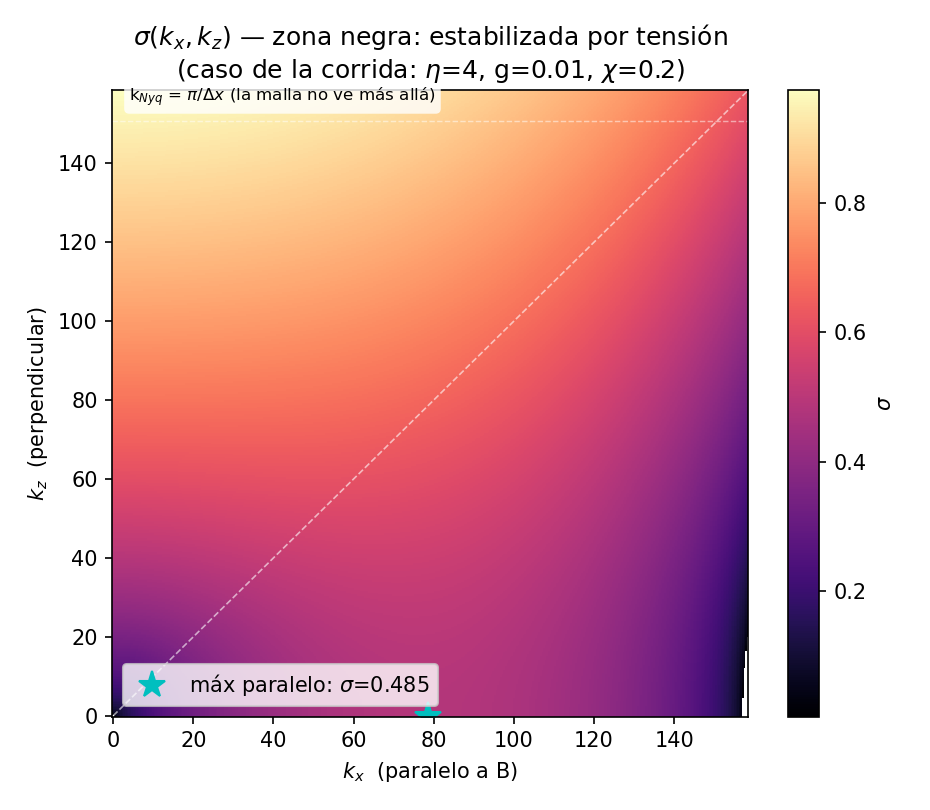
\includegraphics[width=0.62\textwidth]{teoria_mapa_sigma.png}
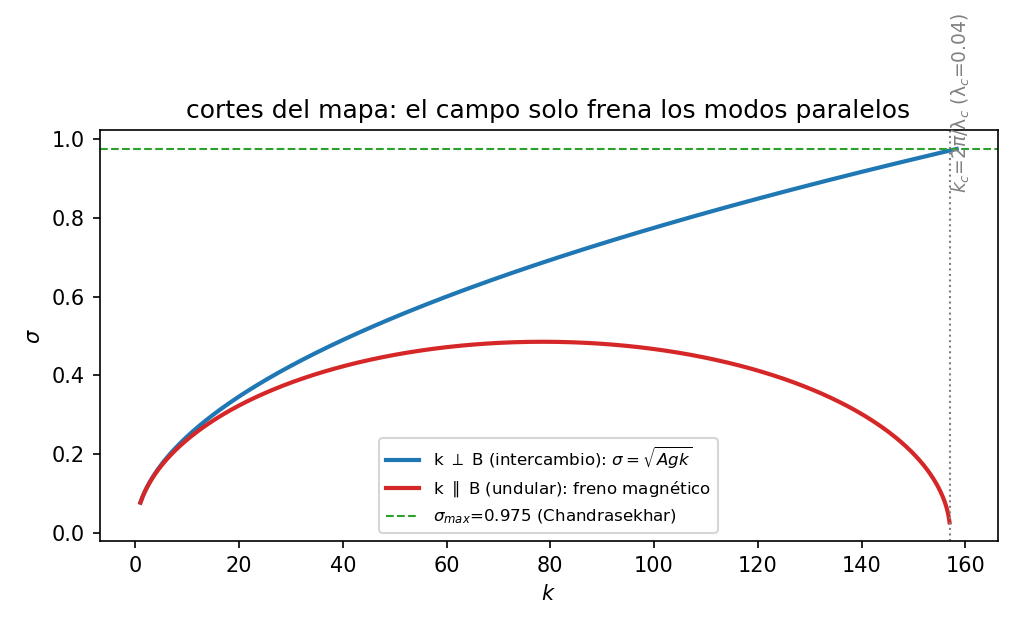
\includegraphics[width=0.62\textwidth]{teoria_cortes.png}
\caption{Arriba: mapa $\sigma(k_x,k_z)$; la zona negra cerca del eje $k_x$ son los modos
estabilizados por la tensión magnética. Abajo: cortes $\parallel$ y $\perp$ al campo.}
\end{figure}

\textbf{El detalle que cambió mi diagnóstico}: comparé $\lambda_c$ con la malla y resultó
que $k_c=2\pi/\lambda_c\approx157$ es apenas MAYOR que el Nyquist ($\approx151$). Es
decir: con $48^3$ celdas, \emph{ningún} modo que la malla ve llega a estar estabilizado
por corte duro; lo que la malla sí ve es la diferencia de \emph{tasas} ($\sigma$ menor
para $k_x$ grande al mismo $|k|$). Por eso el análisis del espectro lo hice por sectores
de ángulo y no buscando un ``hueco'' de estabilidad: el hueco cae fuera de la foto.

\section{Resultados}

\subsection{Morfología: dedos anisótropos}

\begin{figure}[H]
\centering
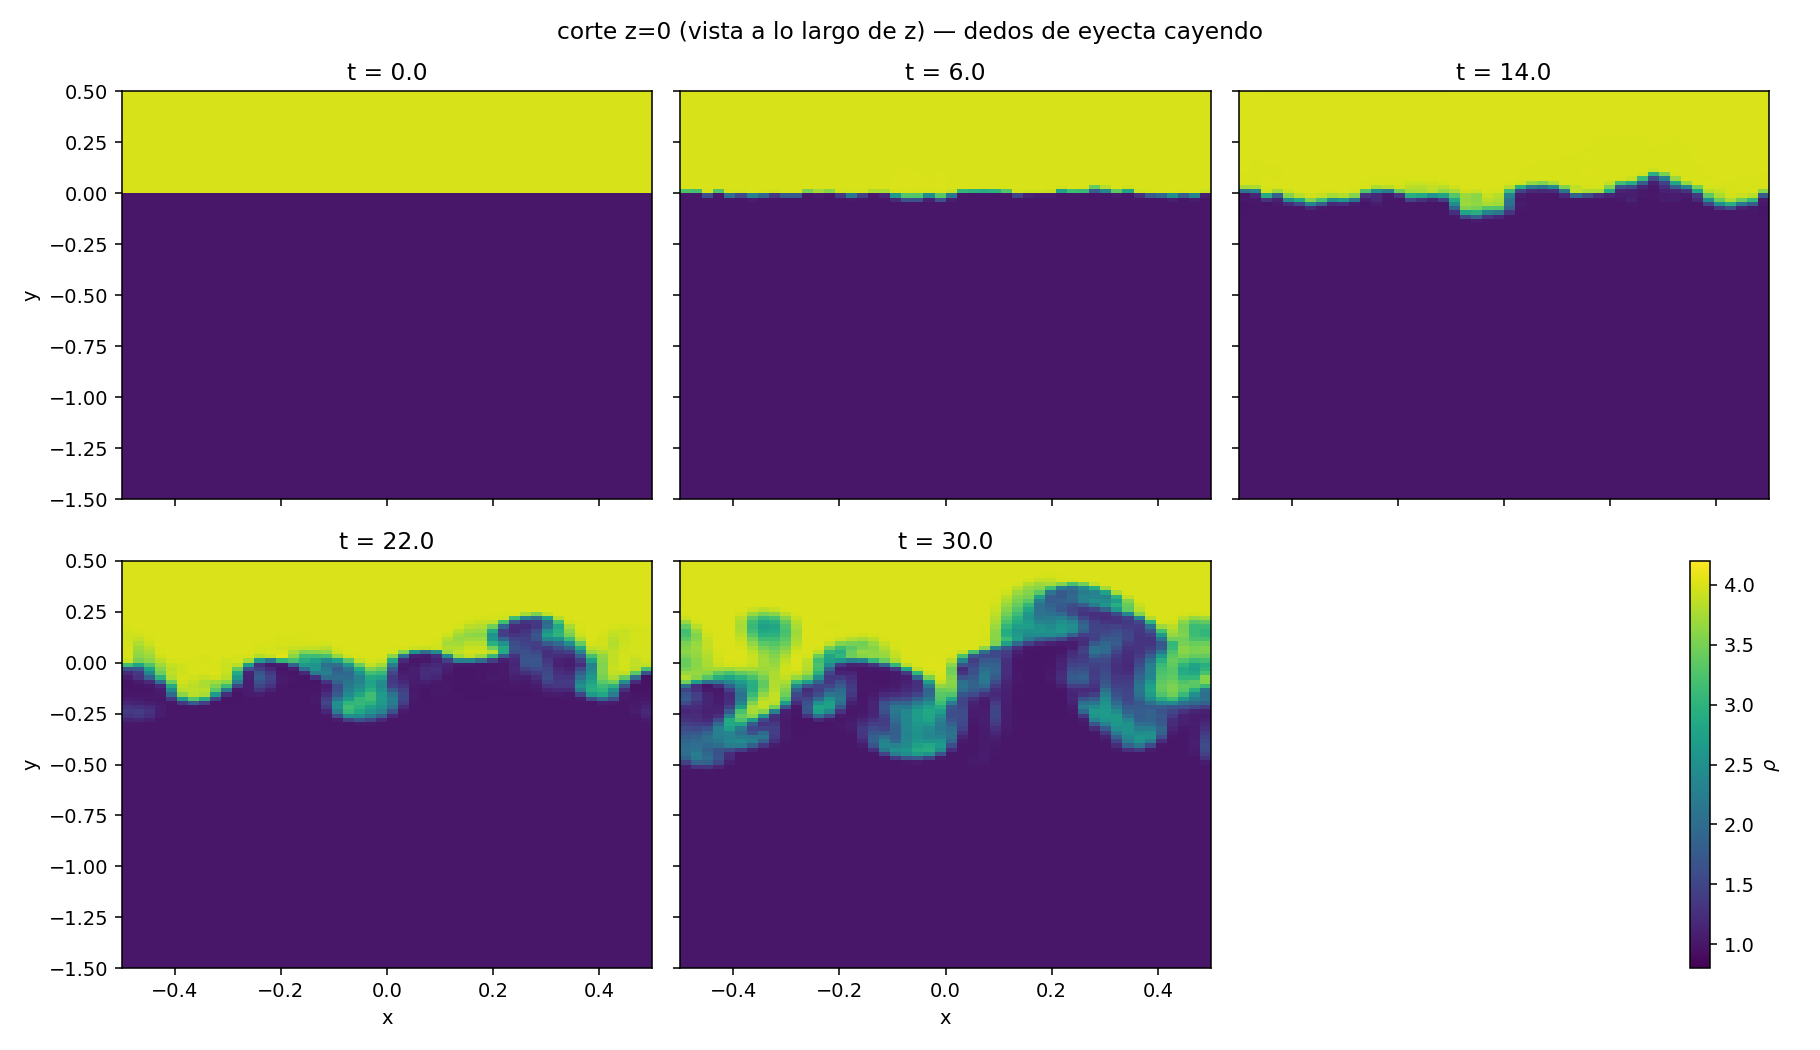
\includegraphics[width=\textwidth]{sim_cortes_yx.png}
\caption{Cortes $z=0$ (mirando a lo largo de $z$) de la densidad. El fluido pesado
($\rho=4$, eyecta) cae en picos y el ligero sube en burbujas.}
\end{figure}

\begin{figure}[H]
\centering
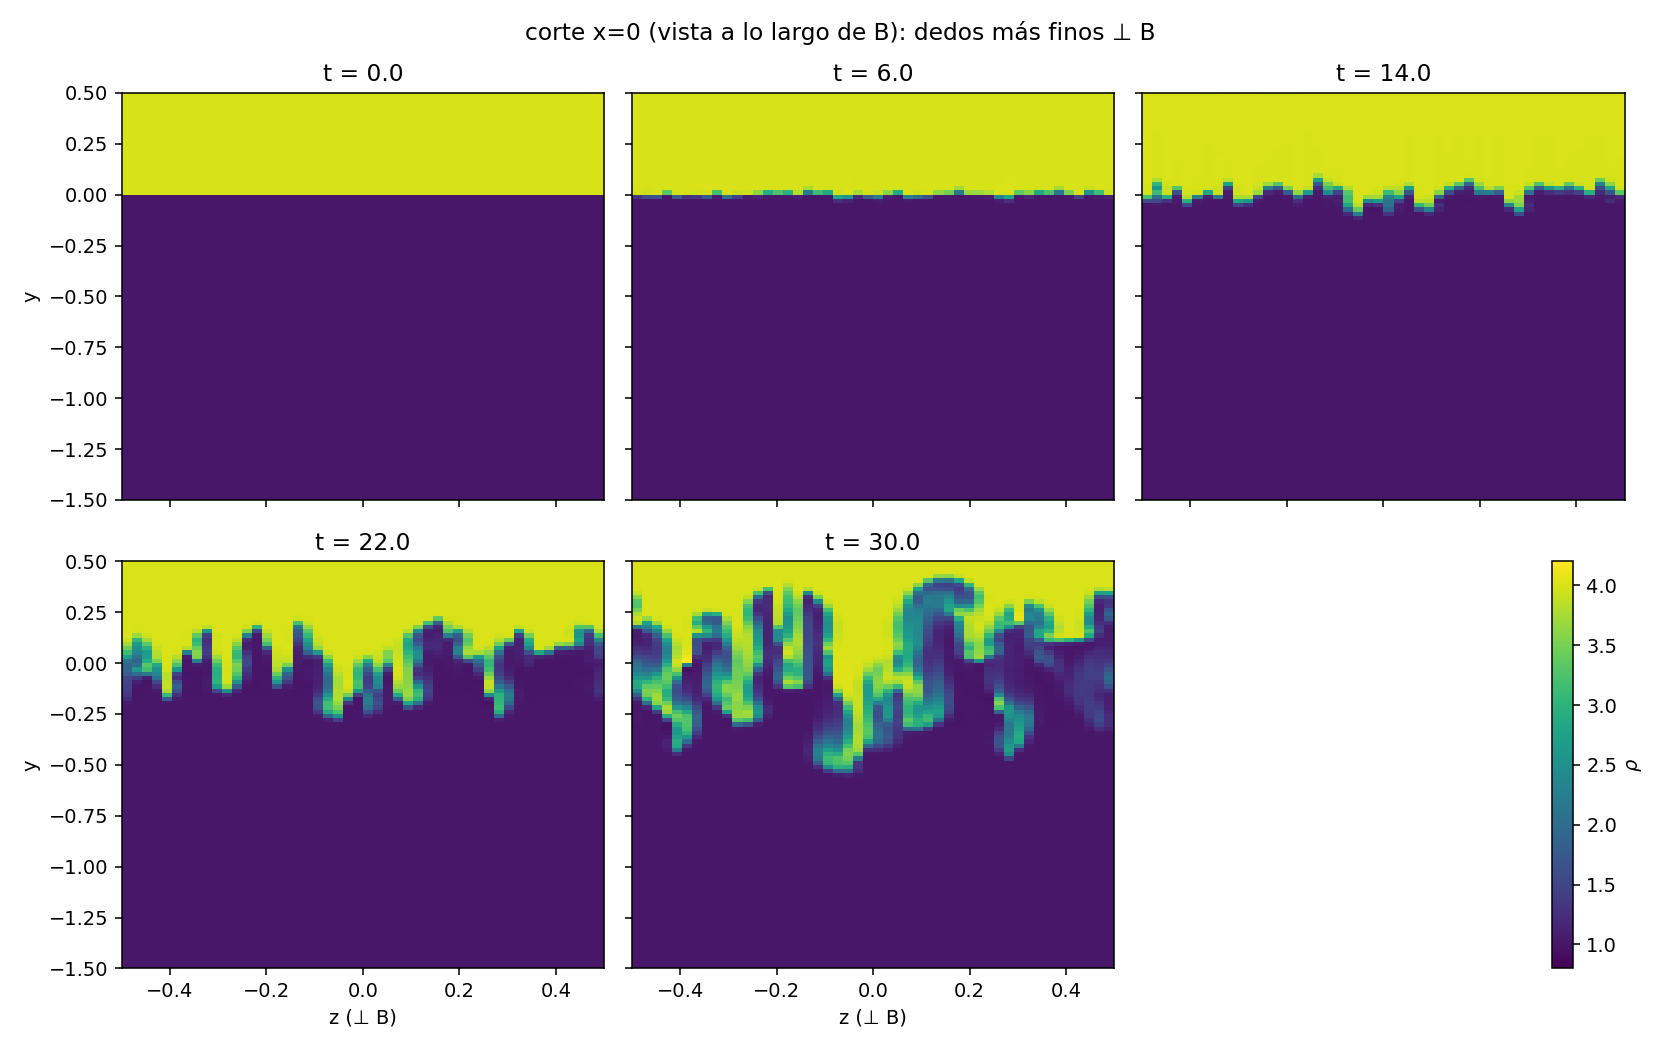
\includegraphics[width=\textwidth]{sim_cortes_yz.png}
\caption{Los mismos instantes en el corte $x=0$, mirando \emph{a lo largo del campo}.}
\end{figure}

Cómo las leo: en el corte $z=0$ la vista mezcla dedos de todas las orientaciones; en el
corte $x=0$ estoy mirando a lo largo de $\mathbf{B}$, así que lo que cruza el plano son
las secciones transversales de los dedos. Lo que esperaba (y salió): transversal al campo
los dedos se ven \emph{más finos y numerosos} --- ahí los modos de intercambio crecen sin
freno --- mientras que a lo largo del campo las estructuras tienden a fusionarse en hojas
largas.

\begin{figure}[H]
\centering
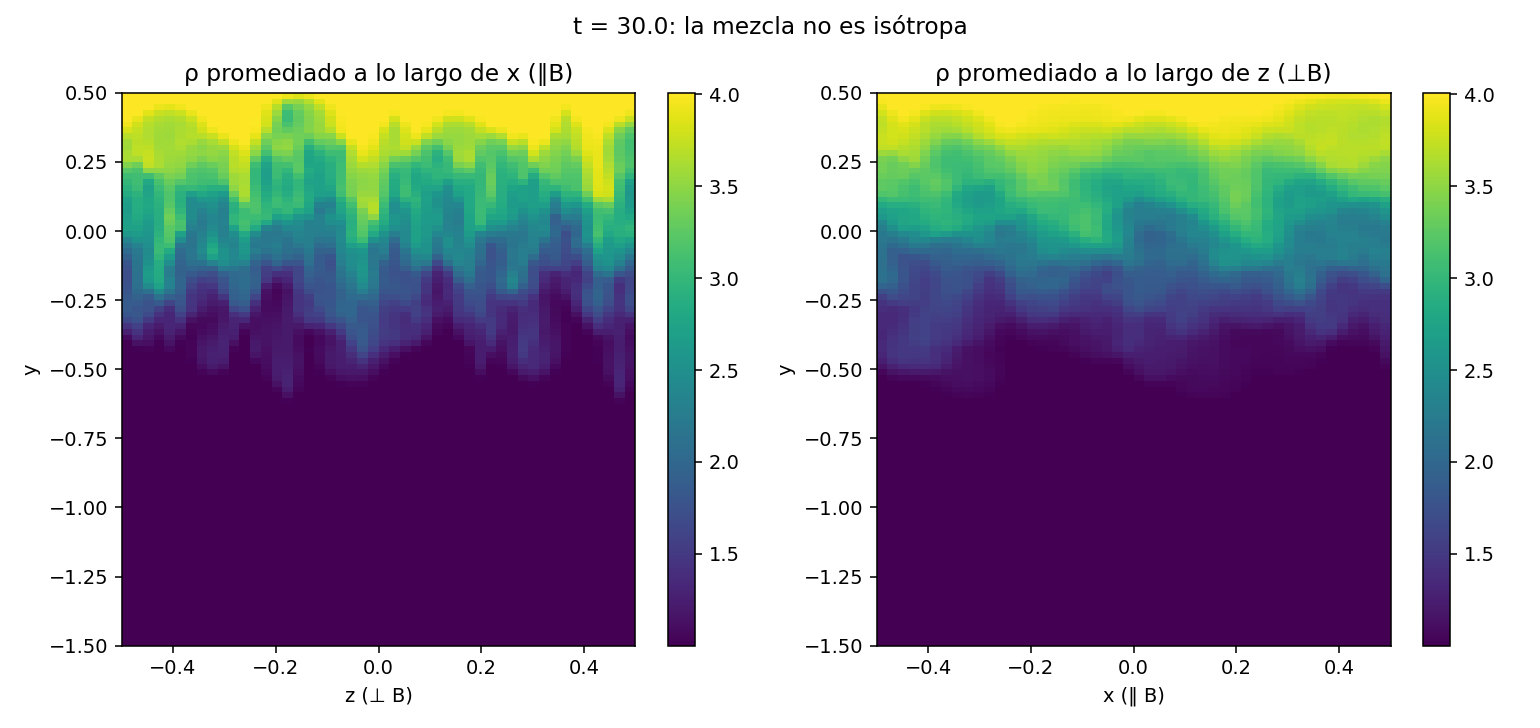
\includegraphics[width=0.9\textwidth]{sim_promedios.png}
\caption{$\rho$ promediado a lo largo de cada eje horizontal en $t=30$.}
\end{figure}

Los promedios son la forma más simple de cuantificar eso: si promedio $\rho$ a lo largo
de $x$ (la dirección de $\mathbf{B}$), todas las estructuras alargadas en esa dirección
se suavizan y quedan las secciones transversales; si promedio a lo largo de $z$, quedan
las hojas alargadas en $x$. La asimetría entre los dos mapas ES la anisotropía
magnética, a simple vista.

\subsection{Crecimiento de la capa de mezcla}

\begin{figure}[H]
\centering
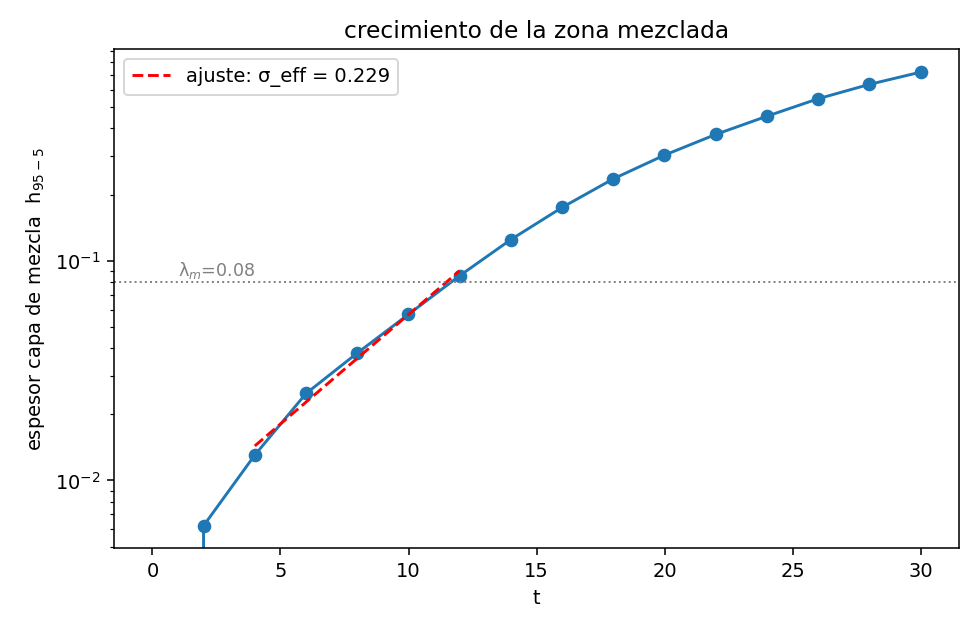
\includegraphics[width=0.62\textwidth]{sim_hmix.png}
\caption{Espesor $h_{95-5}$ de la capa de mezcla. Ajuste en $2\lesssim t\lesssim12$.}
\end{figure}

Para medir el crecimiento sin depender de un solo dedo, el notebook busca todos los
cruces de $\rho=2.5$ (punto medio entre 1 y 4) en cada columna vertical y toma la
distancia entre los percentiles 95 y 5 de su distribución (percentiles y no extremos,
para que un dedo aventurero no infle la medida). El ajuste log-lineal da
$\sigma_\mathrm{eff}\approx \SIGeff$.

Lo interesante es \emph{dónde} cae ese número: dentro del rango teórico
($0.19$--$0.49$) pero cerca del fundamental (0.23), lejos del modo de malla. Mi lectura:
la difusión numérica actúa como una viscosidad efectiva que amputa los modos más finos
(aunque la teoría incompresible los declare los más rápidos), y el crecimiento medible
queda dominado por los modos medianos. Es el mismo efecto por el que una RT simulada
nunca produce estructuras más finas que unas pocas celdas. Después de $t\sim12$ la curva
se aplana: los dedos se fusionan y la capa satura (régimen no lineal tardío, ya no vale
$e^{\sigma t}$).

\subsection{El espectro de la interfaz: la anisotropía medida}

\begin{figure}[H]
\centering
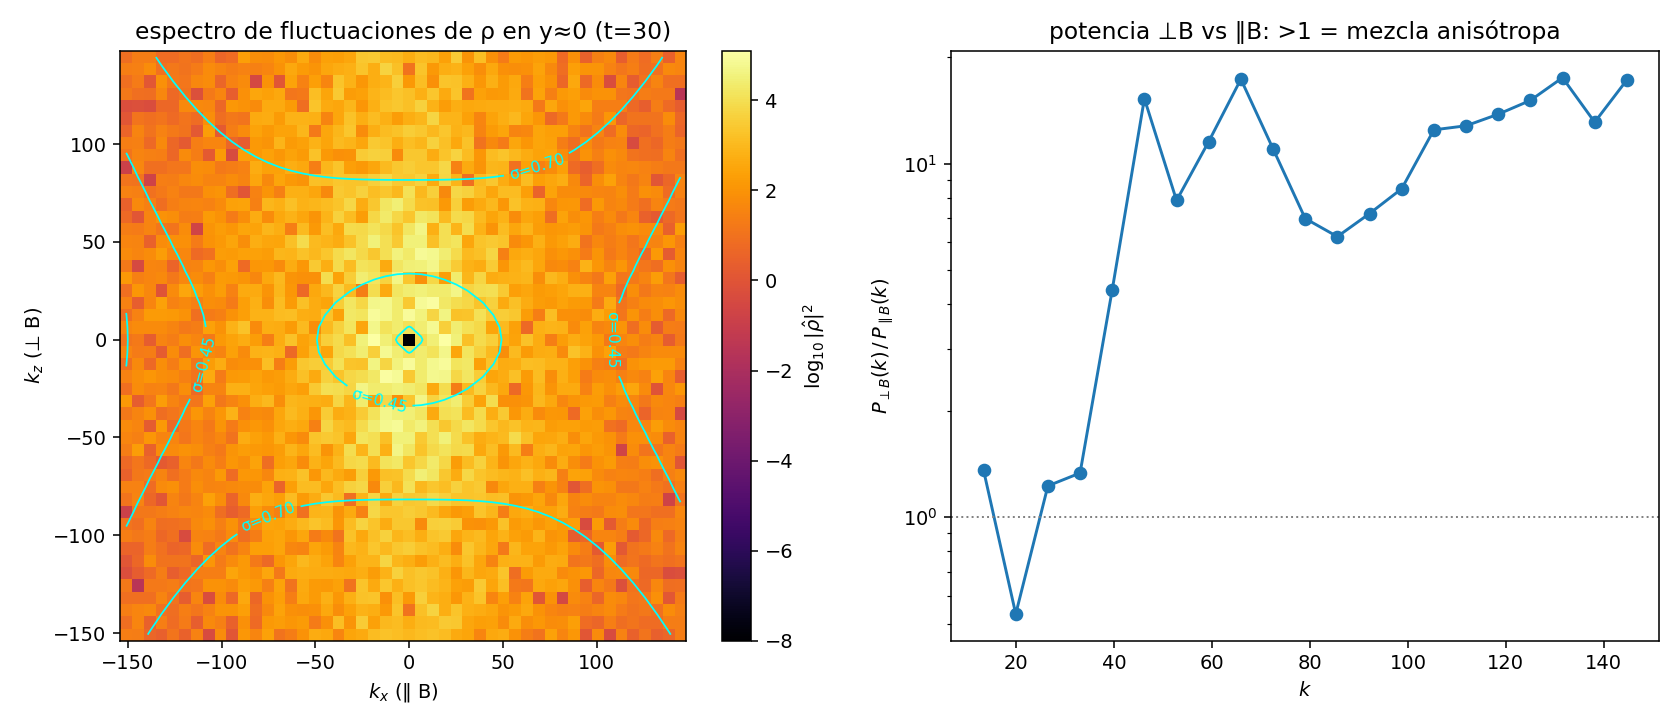
\includegraphics[width=\textwidth]{sim_espectro.png}
\caption{Izquierda: potencia de las fluctuaciones de $\rho$ en la lámina $y\approx0$,
con iso-contornos de $\sigma$ teórico (el borde $\sigma=0$ cae en $k\approx157$, fuera
del rango de la malla). Derecha: razón de potencia en sectores $\pm30^\circ$ alrededor
de $\perp$B y de $\parallel$B.}
\end{figure}

Este es el diagnóstico que mejor condensa la física del proyecto. Tomo una lámina de
$\rho$ pegada a la interfaz, le resto el fondo, hago la FFT 2D en el plano $(x,z)$ y
comparo la potencia en dos sectores de ángulo: alrededor del eje $k_x$
($\parallel\mathbf{B}$, frenado por tensión) y alrededor del eje $k_z$
($\perp\mathbf{B}$, libre). Si el campo hace lo que dice la eq.~\eqref{eq:disp}, en los
$k$ altos la potencia transversal debe dominar.

Salió $P_\perp/P_\parallel\approx17$ en el bin más fino. En palabras: hay del orden de
veinte veces más estructura fina transversal al campo que paralela a él. Con esa medida,
la anisotropía de las figuras de morfología deja de ser impresión visual y pasa a ser un
número, consistente con el mecanismo de tensión magnética (y con lo que reportan las
simulaciones 3D de SNR \cite{orlando2012} y prominencias \cite{hillier2012}).

\subsection{Energías y divergencia: los chequeos de honestidad}

\begin{figure}[H]
\centering
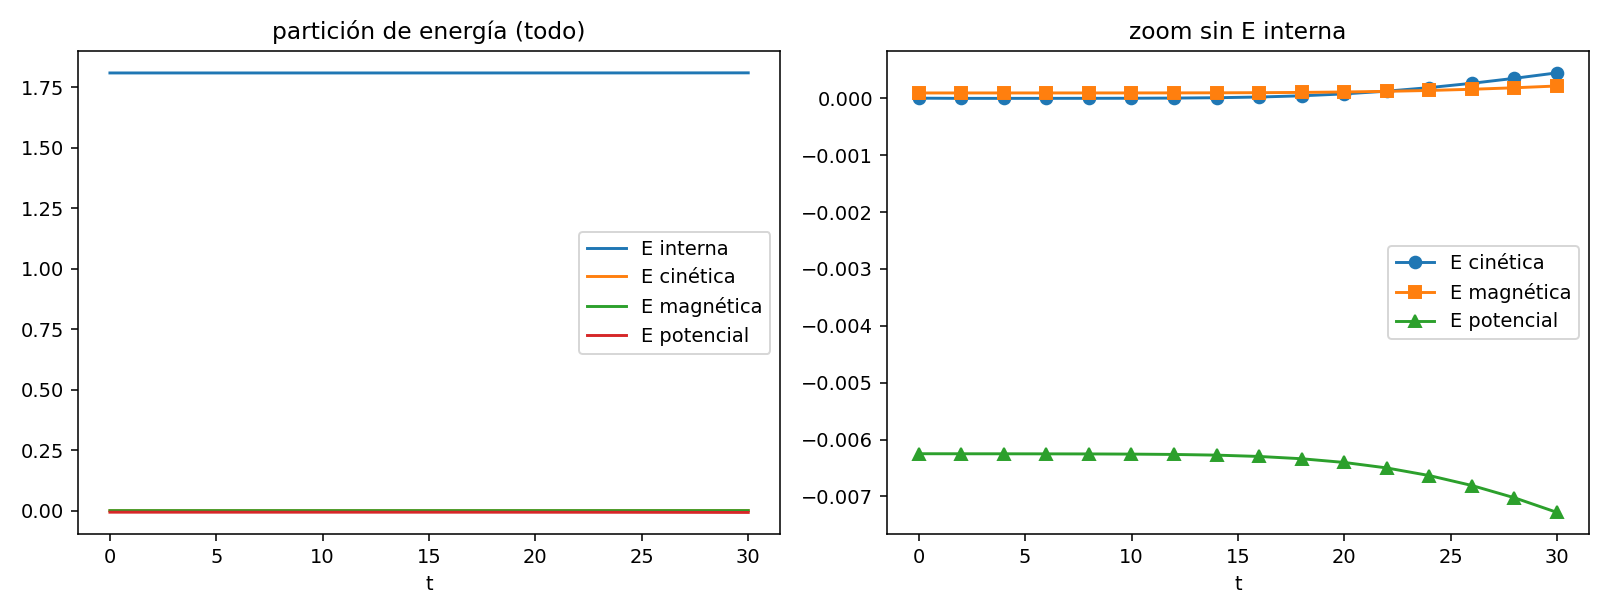
\includegraphics[width=\textwidth]{sim_energias.png}
\caption{Partición de energía. Izquierda: las cuatro; derecha: zoom sin $E_\mathrm{interna}$
(que vale $\sim1.75$ y aplastaría la escala).}
\end{figure}

Qué debería pasar: en el dominio cerrado (paredes reflectivas) la energía total
$E_\mathrm{int}+E_\mathrm{cin}+E_\mathrm{mag}+E_\mathrm{pot}$ se conserva, y la
inestabilidad convierte potencial gravitacional en cinética (y algo en magnética, por el
estiramiento de líneas). Es lo que se ve: $E_\mathrm{pot}$ cae, $E_\mathrm{cin}$ sube
casi como su espejo, $E_\mathrm{mag}$ crece (amplificación por estiramiento en las
puntas). La deriva total medida fue $\sim\EDRIFT$ relativa a $|E_\mathrm{pot}(0)|$:
conservación a nivel de épsilon de máquina, que valida el esquema conservativo con la
fuente gravitacional bien puesta.

\begin{figure}[H]
\centering
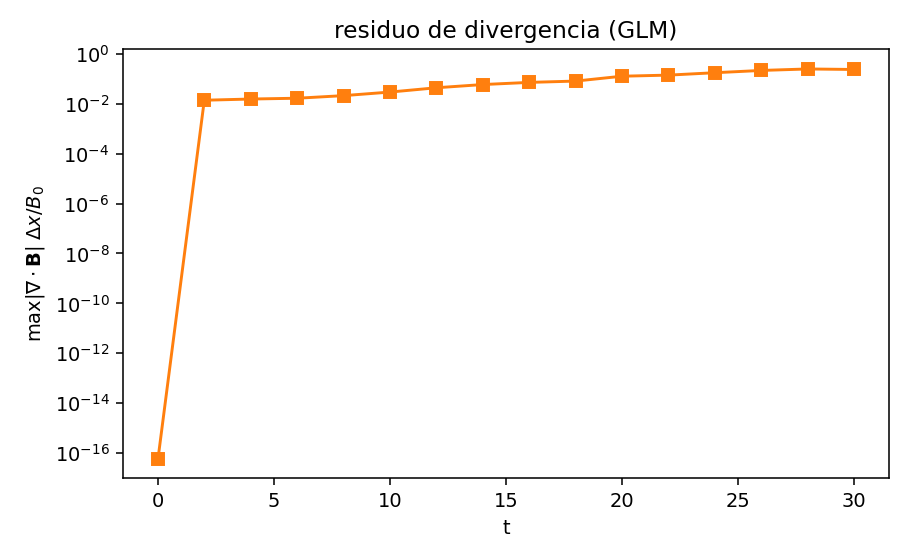
\includegraphics[width=0.55\textwidth]{sim_divB.png}
\caption{Residuo de divergencia (GLM) en el tiempo.}
\end{figure}

Con GLM el $\nabla\cdot\mathbf{B}$ residual llega a $\sim\DIVBfin$ al final de la corrida
en unidades de $B_0/\Delta x$, con $B_0$ el campo \emph{inicial}. Dos comentarios que me
tomó un rato entender: (i) referirlo al campo inicial infla el número, porque el campo
local se amplifica por estiramiento (el mismo crecimiento de $E_\mathrm{mag}$ de la
figura anterior); relativo al campo real es un orden de magnitud menos; (ii) con la
config 2D de CT este número sería $\sim10^{-15}$: esa es la diferencia de precio entre
\#09 y \#07, y es chico para lo que le pido a esta corrida.

\section{Limitaciones y lo que seguiría}

\begin{itemize}[nosep]
  \item \textbf{Una sola malla}. $\lambda_c=0.04$ son $\sim2$ celdas: la escala de corte
  magnético está apenas resuelta (y el corte duro, ni eso: cae fuera de Nyquist). Una
  malla $96\times192\times96$ sería $\sim8\times$ más cara ($\sim$3 h) y dejaría el corte
  adentro de la foto. El $\sigma_\mathrm{eff}$ medido probablemente está subestimado por
  difusión numérica.
  \item \textbf{Sin control $\chi=0$}: la anisotropía medida es consistente con la
  teoría, pero la forma limpia de aislarla sería correr el mismo setup sin campo y
  comparar espectros. Queda para la siguiente versión, junto con un barrido en $\chi$.
  \item \textbf{Gravedad constante vs.\ real}: en el SNR $|a|\propto t^{\eta-2}$ decae;
  aquí es constante. Es la aproximación de parche local estándar, pero conviene decirlo.
  \item \textbf{Una sola lámina para el espectro}: promediar unas pocas láminas alrededor
  de $y=0$ bajaría el ruido del espectro sin costo.
\end{itemize}

\section{Bibliografía que usé para esta parte}

\begin{thebibliography}{9}\small
\bibitem{orlando2012} Orlando, S. et al.\ 2012, ``3D MHD simulations of a magnetized
supernova remnant'' (arXiv:1202.3593).
\bibitem{fraschetti2010} Fraschetti, F. et al.\ 2010, ``Simulation of the growth of the
3D Rayleigh--Taylor instability in young supernova remnants'' (arXiv:1002.5048).
\bibitem{warren2013} Warren, D.~C. \& Blondin, J.~M. 2013, MNRAS 429, 3099.
\bibitem{chandra1961} Chandrasekhar, S. 1961, \emph{Hydrodynamic and Hydromagnetic
Stability}, caps.~X.
\bibitem{sg2007} Stone, J.~M. \& Gardiner, T.~A. 2007, Phys.\ Fluids 19, 094104
(la referencia del problema 2D del proyecto).
\bibitem{hillier2012} Hillier, A. et al.\ 2012, ApJ 746, 120 (RT magnético 3D en
prominencias; misma física de modos de intercambio).
\bibitem{mignone2012} Mignone, A. et al.\ 2012, ApJS 198, 7 (PLUTO, y el GLM de la
config \#09 en Mignone et al.\ 2010, JCP 229, 2117).
\end{thebibliography}

\end{document}
